\chapter{Ewaluacja}
\label{cha:ewaluacja}

%---------------------------------------------------------------------------

\section{Na czym polega ewaluacja?}
\label{sec:naCzymPolegaEwaluacja}

Kolejnym etapem, po zaprojektowaniu i zaimplementowaniu aplikacji była ewaluacja zapopononowanego rozwiązania, czyli zebranie opinii o wartości działania programu poprzez przeprowadzenie badania wśród użytkowników. 

Należy przypomnieć, że celem pracy było zaprojektowanie, implementacja i ewaluacja mechanizmu pozyskiwania wiedzy o  stanie emocjonalnym użytkownika w systemach \textit{affective computing}. Na potrzeby pracy zaprojektowana i zaimplementowana została aplikacja mobilna pozwalająca na uczynienie jawnej mediacji wiedzy możliwie nieintruzywną (poprzez wnioskowanie oparte na monitorowaniu czynników zewnętrznych) oraz na przeprowadzenie niejawnej mediacji (z wykorzystaniem aparatu fotograficznego telefonu). 

Ewaluację przeprowadzono w formie badania. Zebrano grupę osób, po czym na ich telefonach komórkowych zainstalowano aplikację wykorzystującą różne metody mediacji wiedzy. Po zakończeniu kilkudniowego etapu testowania aplikacji, każdy z uczestników otrzymał listę pytań, na które należało udzielić odpowiedzi. Pytania (opisane w sekcji trzeciej niniejszego rozdziału) skostruowano w ten sposób, aby potwierdzić założenia pracy i obserwacje wysnute podczas etapów projektowania i implementacji. Jeżeli odpowiedzi na pytania potwierdzą te hipotezy, będzie to oznaczało, że rozwiązanie w formie aplikacji mobilnej \textit{HowAreYou} spełnia swoje podstawowe zadania.

%---------------------------------------------------------------------------

\section{Sposób przeprowadzenia badania}
\label{sec:sposobPrzeprowadzeniaBadania}

Badanie przeprowadzono na grupie mężczyzn i kobiet w wieku 22-27 lat uruchamiając na ich telefonach aplikację \textit{AWARE} wraz z pluginem \textit{HowAreYou}. Zadaniem osób badanych było korzystanie z~telefonu tak, jak to czynią na co dzień. Należy jednak podkreślić, że uruchomiona w tle aplikacja przeprowadzała badanie nastroju wchodząc w interakcję z użytkownikiem poprzez pytanie o emocje, o kolor i wykonywanie fotografii.

Dziewięciorgu uczestnikom zaproponowano korzystanie z zaawansowanej wersji aplikacji (wzbogaconej o inteligentne wnioskowanie w oparciu o większą liczbę tzw. \textit{callbacks}). W ich przypadku plugin połączony został ze \textit{study}, a zebrane dane zgromadzone zostały w bazie danych MySQL. W bazie nie gromadzono fotografii, a jedynie anonimowe dane o stanie emocjonalnyn i informacje, które były wykorzystywane przez silnik wnioskujący.

Dla porównania kolejnym czworgu uczestnikom zapropono wykorzystanie wersji uproszczonej (pytającej o nastrój w regularnych odstępach).

Następnie skonstruowano formularze kwestionariuszy użytkownika, także w dwóch wersjach. Co naturalane, formularz dla osób z pierwszej grupy zawierał dodatkowe pytania, które pozwoliły ocenić działanie wersji rozszerzonej.

Odpowiedzi mogły być udzielone na jednakowej, pięciopunktowej skali:
\begin{itemize}
	\item zdecydowanie się nie zgadzam, 
	\item raczej się nie zgadzam,
	\item nie mam zdania,
	\item raczej się zgadzam,
	\item zdecydowanie się zgadzam.
\end{itemize}

Każda z powyższych wartości miała przypisaną wartość całkowitą: od -2 do +2.

Odpowiedzi na każde z pytań poddano prostej analizie statystycznej -- dla każdego obliczono wartość średnią, wariancję i medianę. Wyniki zaokrąglono matematycznie do dwóch miejsc po przecinku.

Dla każdego z pytań dane przedstawiono na wykresie pudełkowym (ang. boxplot). Na płaszczyźnie umieszczono niebieski prostokąt, którego dolny bok jest wyznaczony przez pierwszy kwartyl, a prawy bok przez trzeci kwartyl. Dodatkowe ,,wąsy'' poza prostokątem wskazują najmniejszą i największą wartość w zbiorze. Czerwona pionowa linia wewnątrz prostokąta określa wartość mediany.

%---------------------------------------------------------------------------

\section{Konstrukcja kwestionariuszy i ewaluacja wyników badania}
\label{sec:konstrukcjaKwestionariuszyIEwaluacjaWynikowBadania}

W celu przeprowadzenia badania, przygotowano kwestionariusz zawierający następujące pytania:

\subsection{Czy system był wygodny w użyciu?}

	\subsubsection{Cel pytania:}
	
	Celem pytania była ogólna ocena zachowania aplikacji.
	\clearpage
	
	\subsubsection{Uzyskane wyniki:}
	
	\begin{table}[!h]
		\caption{Ewaluacja: pytanie 1 -- uzyskane wyniki.}
		\centering
		\begin{tabular}{|c|c|c|c|c|c|c|c|c|c|c|c|c|c|}
			\hline
			Wersja &  \multicolumn{9}{c|}{Zaawansowana} & \multicolumn{4}{c|}{Uproszczona}\\ \hline
			Identyfikator użytkownika             & 1 & 2 & 3 & 4 & 5 & 6 & 7 & 8 & 9 
			                                      & 10 & 11 & 12 & 13 \\ \hline
			Odpowiedzi poszczególnych uczestników & 2 & 1 & 2 & 2 & 2 & 1 & 1 & 0 & 2 
			                                      & 0 & 1 & 2 & 1     \\ \hline
		\end{tabular}
	\end{table}

	\begin{table}[!h]
		\caption{Ewaluacja: pytanie 1 -- prosta analiza statystyczna.}
		\centering
		\begin{tabular}{|c|c|c|}
			\hline
			Wersja          & Zaawansowana & Uproszczona \\ \hline
			Wartość średnia & 1.44         & 1.00        \\ \hline
			Wariancja       & 0.53         & 0.67        \\ \hline
			Mediana         & 2.00         & 1.00        \\ \hline
		\end{tabular}
	\end{table}

	\begin{figure}[H]
		\centering
		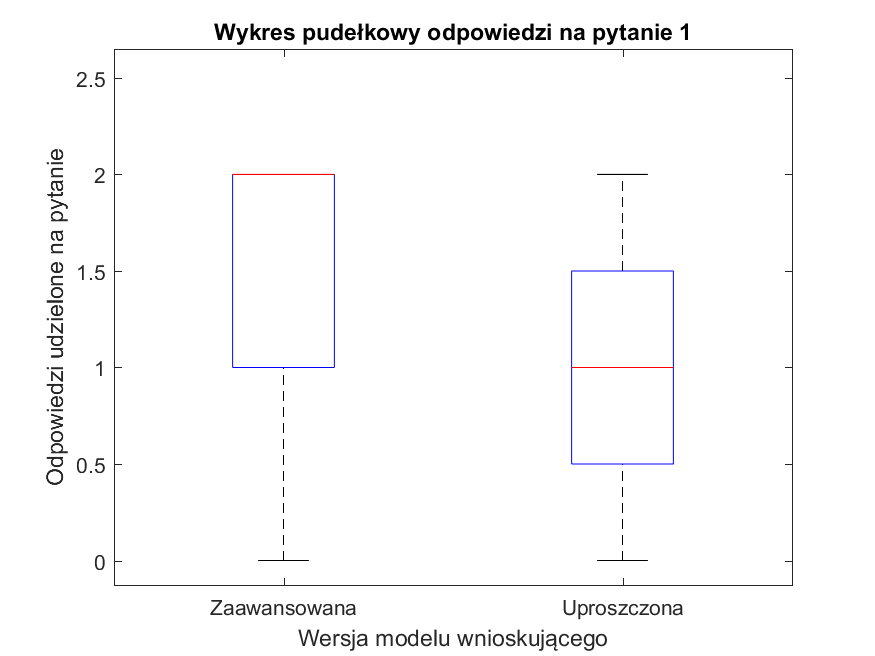
\includegraphics[scale=0.8]{rozdzial5/Ewaluacja1.png}
		\caption{Ewaluacja: pytanie 1 -- wykres pudełkowy.}
	\end{figure}
	
	\subsubsection{Obserwacje i wnioski:}
	
	Statystycznie nieco bardziej z całokształtu zadowoleni byli użytkownicy wersji zaawansowanej, stanowiącej podstawę niniejszczego badania. Całokształt ogólnego zachowania aplikacji został oceniony przez użytkowników dobrze -- z medianą 2 dla wersji zaawansowanej.


\subsection{Czy system pytał mnie o nastrój w nieodpowiednich momentach?}

	\subsubsection{Cel pytania:}
	
	Odpytywanie użytkownika musiało być najbardziej uciążliwą czynnością. Wszystkie inne działania pluginu \textit{HowAreYou} były wykonywane w tle. Celem zaawansowanej wersji było zmniejszenie tej uciążliwości.
	
	\subsubsection{Uzyskane wyniki:}
	
	\begin{table}[!h]
		\caption{Ewaluacja: pytanie 2 -- uzyskane wyniki.}
		\centering
		\begin{tabular}{|c|c|c|c|c|c|c|c|c|c|c|c|c|c|}
			\hline
			Wersja &  \multicolumn{9}{c|}{Zaawansowana} & \multicolumn{4}{c|}{Uproszczona}\\ \hline
			Identyfikator użytkownika             & 1 & 2 & 3 & 4 & 5 & 6 & 7 & 8 & 9 
			& 10 & 11 & 12 & 13 \\ \hline
			Odpowiedzi poszczególnych uczestników & -1 & -2 & 0 & 1 & -1 & -1 & 1 & 2 & 0
			& 2 & 1 & 2 & 1     \\ \hline
		\end{tabular}
	\end{table}
	
	\begin{table}[!h]
		\caption{Ewaluacja: pytanie 2 -- prosta analiza statystyczna.}
		\centering
		\begin{tabular}{|c|c|c|}
			\hline
			Wersja          & Zaawansowana & Uproszczona \\ \hline
			Wartość średnia & -0.11        & 1.50        \\ \hline
			Wariancja       &  1.61        & 0.33        \\ \hline
			Mediana         &  0.00        & 1.50        \\ \hline
		\end{tabular}
	\end{table}
	
	\begin{figure}[H]
		\centering
		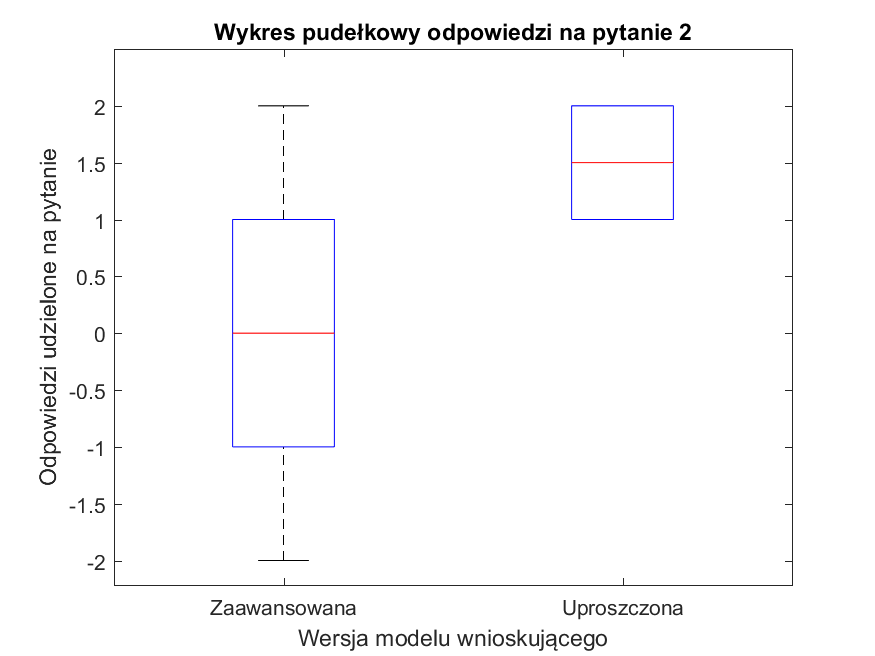
\includegraphics[scale=0.8]{rozdzial5/Ewaluacja2.png}
		\caption{Ewaluacja: pytanie 2 -- wykres pudełkowy.}
	\end{figure}
	
	\subsubsection{Obserwacje i wnioski:}
	
	Wyniki dla użytkowników podstawowej wersji aplikacji okazały się być bardzo zróżnicowane. Część badanych wskazała, że odpytywanie o nastrój im nie przeszkadzało. Pojawiły się też niestety głosy, że było to jednak irytujące. Inaczej sytuacja wygląda, jeżeli chodzi o odpowiedzi osób, wykorzystujących wersję klasyczną (z regularnym odpytywaniem) -- tutaj wszyscy użytkownicy wskazali, że byli pytani w nieodpowiednich momentach. Dzięki wykorzystaniu silnika wnioskującego i sensorów udało się więc ograniczyć w znaczący sposób uciążliwość odpytywania użytkownika.
	
	
	\subsection{Czy miałem wątpliwości jak odpowiadać na pytania o odczuwane przez siebie emocje?}
	
	\subsubsection{Cel pytania:}
	
	W tym pytaniu chodziło o sprawdzenie, jak użytkownicy odbierają wygląd i sposób działania aktywności z widokiem emotikon. Warto podkreślić, że widok emotikon został zachowany w sposób identyczny w~wersji B.
	
	\subsubsection{Uzyskane wyniki:}
	
	\begin{table}[!h]
		\caption{Ewaluacja: pytanie 3 -- uzyskane wyniki.}
		\centering
		\begin{tabular}{|c|c|c|c|c|c|c|c|c|c|c|c|c|c|}
			\hline
			Wersja &  \multicolumn{9}{c|}{Zaawansowana} & \multicolumn{4}{c|}{Uproszczona}\\ \hline
			Identyfikator użytkownika             & 1 & 2 & 3 & 4 & 5 & 6 & 7 & 8 & 9 
			& 10 & 11 & 12 & 13 \\ \hline
			Odpowiedzi poszczególnych uczestników & -2 & -1 & -1 & -1 & 0 & -2 & -1 & -2 & -1
			& -1 & 0 & -2 & -1  \\ \hline
		\end{tabular}
	\end{table}
	
	\begin{table}[!h]
		\caption{Ewaluacja: pytanie 3 -- prosta analiza statystyczna.}
		\centering
		\begin{tabular}{|c|c|c|}
			\hline
			Wersja          & Zaawansowana & Uproszczona \\ \hline
			Wartość średnia & -1.22        & -1.00       \\ \hline
			Wariancja       &  0.44        &  0.67       \\ \hline
			Mediana         & -1.00        & -1.00       \\ \hline
		\end{tabular}
	\end{table}
	\clearpage
	
	\begin{figure}[H]
		\centering
		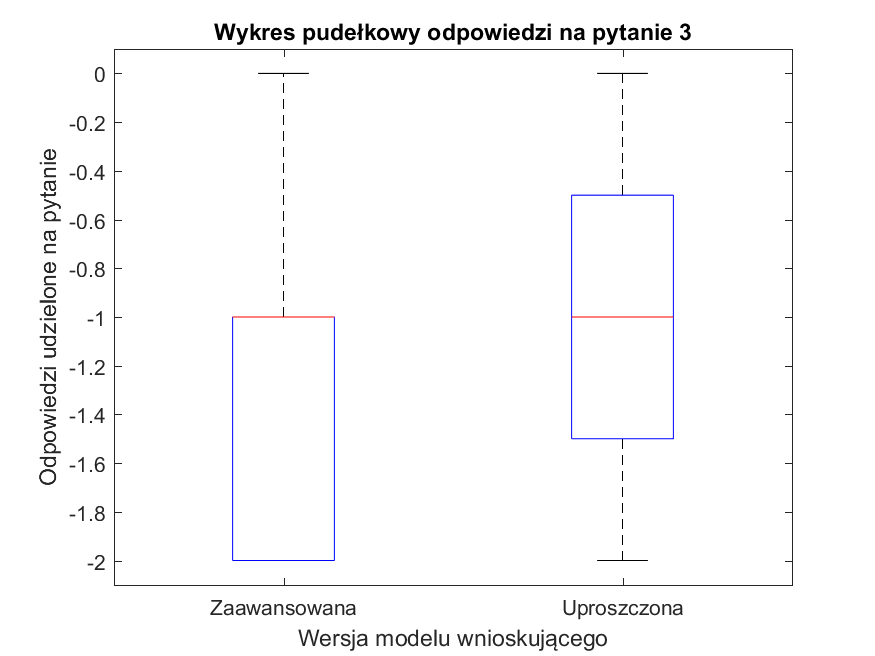
\includegraphics[scale=0.8]{rozdzial5/Ewaluacja3.png}
		\caption{Ewaluacja: pytanie 3 -- wykres pudełkowy.}
	\end{figure}
	
	\subsubsection{Obserwacje i wnioski:}
	
	Użytkownikom przypadło do gustu odpytywanie z wykorzystaniem widoku emotikon. Badani z obydwu grup wskazali w przeważającej większości, że nie mieli wątpliwości, jak odpowiadać na zadane pytania.
	
	
	\subsection{Czy miałem wątpliwości jak odpowiadać na pytania systemu o kolor odpowiadający temu, jak się czuję?}
	
	\subsubsection{Cel pytania:}
	
	W tym pytaniu chodziło o sprawdzenie, jak użytkownicy odbierają wygląd i sposób działania aktywności z widokiem mapy kolorów. Pytanie nie zostało zadane użytkownikom wersji B.
	
	\subsubsection{Uzyskane wyniki:}
	
	\begin{table}[!h]
		\caption{Ewaluacja: pytanie 4 -- uzyskane wyniki.}
		\centering
		\begin{tabular}{|c|c|c|c|c|c|c|c|c|c|c|c|c|c|}
			\hline
			Wersja &  \multicolumn{9}{c|}{Zaawansowana} & \multicolumn{4}{c|}{Uproszczona}\\ \hline
			Identyfikator użytkownika             & 1 & 2 & 3 & 4 & 5 & 6 & 7 & 8 & 9 
			& 10 & 11 & 12 & 13 \\ \hline
			Odpowiedzi poszczególnych uczestników & 2 & -2 & 1 & 1 & 2 & -2 & 1 & 2 & 0
			& --  & -- & -- & --     \\ \hline
		\end{tabular}
	\end{table}
	
	\begin{table}[!h]
		\caption{Ewaluacja: pytanie 4 -- prosta analiza statystyczna.}
		\centering
		\begin{tabular}{|c|c|c|}
			\hline
			Wersja          & Zaawansowana & Uproszczona \\ \hline
			Wartość średnia & 0.56         & --          \\ \hline
			Wariancja       & 2.53         & --          \\ \hline
			Mediana         & 1.00         & --          \\ \hline
		\end{tabular}
	\end{table}
	
	\begin{figure}[H]
		\centering
		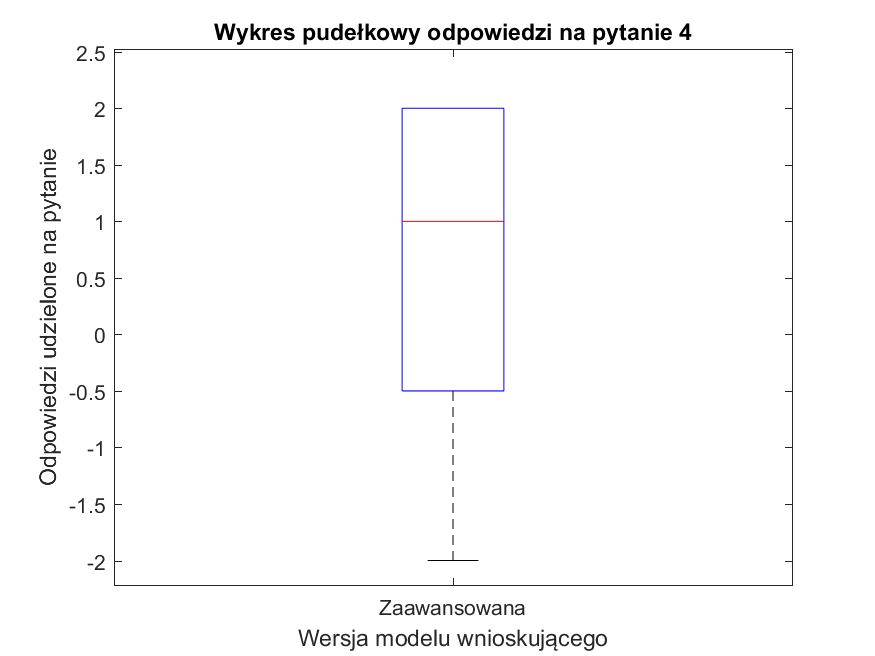
\includegraphics[scale=0.8]{rozdzial5/Ewaluacja4.png}
		\caption{Ewaluacja: pytanie 4 -- wykres pudełkowy.}
	\end{figure}
	
	\subsubsection{Obserwacje i wnioski:}
	
	Zdecydowana większość użytkowników wskazała, że miała problem przy odpowiadaniu na pytania dotyczące koloru. Może to oznaczać, że pytanie ludzi o kolor nie jest dobrym pomysłem. Istnieje ryzyko, że część spośród udzielonych odpowiedzi mogła być losowa -- spowodowana prostym kliknięciem w ekran, aby ,,pozbyć się'' uciążliwego pytania. Całkiem prawdopodobne, że potrzeba bardzo dużo danych, aby z wyników pytania o kolor wysnuć jakieś wnioski. Warto również podkreślić, że odpowiedzi znacznie różnią się miedzy sobą -- u części osób na przykład zdecydowanie wątpliwości się nie pojawiły.



\subsection{Czy określił(a) bym siebie jako umysł ścisły (inżynierski, itp.)?}

	\subsubsection{Cel pytania:}
	
	Pytanie zadano jako uzupełnienie poprzedniego. Chodziło o to, aby zdobyć chociaż namiastkę zrozumienia, jak charakter i osobowość człowieka wpływa na udzielane przez niego odpowiedzi. 
	
	\subsubsection{Uzyskane wyniki:}
	
	\begin{table}[!h]
		\caption{Ewaluacja: pytanie 5 -- uzyskane wyniki.}
		\centering
		\begin{tabular}{|c|c|c|c|c|c|c|c|c|c|c|c|c|c|}
			\hline
			Wersja &  \multicolumn{9}{c|}{Zaawansowana} & \multicolumn{4}{c|}{Uproszczona}\\ \hline
			Identyfikator użytkownika             & 1 & 2 & 3 & 4 & 5 & 6 & 7 & 8 & 9 
			& 10 & 11 & 12 & 13 \\ \hline
			Odpowiedzi poszczególnych uczestników & 1 & -2 & 2 & 2 & 0 & -2 & 2 & 2 & -1
			& --  & -- & -- & --    \\ \hline
			Odpowiedzi na poprzednie pytanie      & 2 & -2 & 1 & 1 & 2 & -2 & 1 & 2 & 0
			& --  & -- & -- & --    \\ \hline
		\end{tabular}
	\end{table}
	
	\begin{table}[!h]
		\caption{Ewaluacja: pytanie 5 -- prosta analiza statystyczna.}
		\centering
		\begin{tabular}{|c|c|c|}
			\hline
			Wersja          & Zaawansowana & Uproszczona \\ \hline
			Wartość średnia & 0.44         & --          \\ \hline
			Wariancja       & 3.03         & --          \\ \hline
			Mediana         & 1.00         & --          \\ \hline
		\end{tabular}
	\end{table}
	
	\begin{figure}[H]
		\centering
		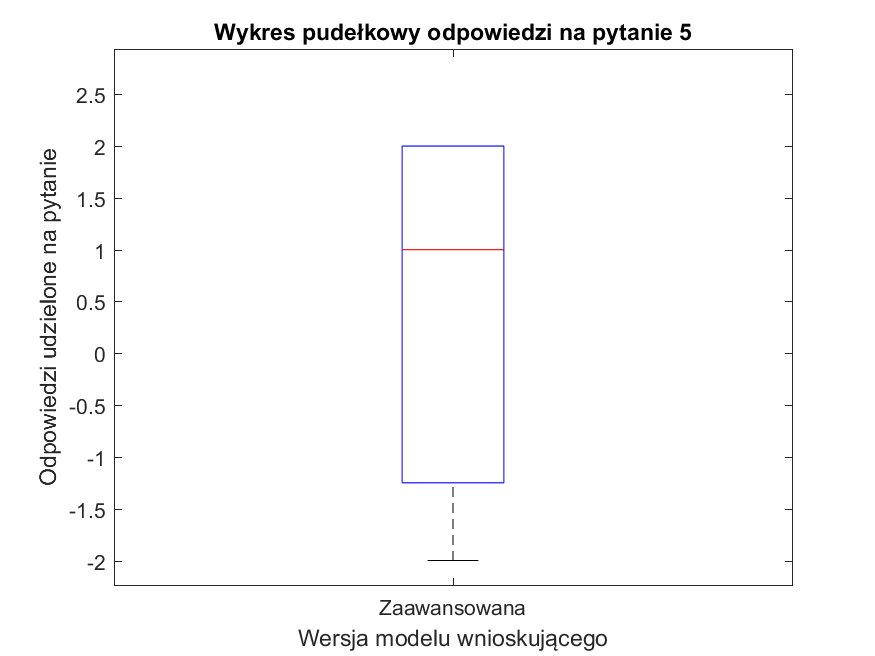
\includegraphics[scale=0.8]{rozdzial5/Ewaluacja5.png}
		\caption{Ewaluacja: pytanie 5 -- wykres pudełkowy.}
	\end{figure}
	
	\subsubsection{Obserwacje i wnioski:}
	
	Większość uczestników testu to inżynierowie. Prawdopodobnie naturalnie więc określili oni siebie jako umysły ścisłe. W teście wzięły też udział osoby o innych zainteresowaniach -- na przykład absolwentka ASP czy studentka medycyny. Pojawiły się więc również odpowiedzi negatywne. Co kluczowe przy tym pytaniu, tak jak przypuszczano, pomimo małej próbki można dostrzec nieznaczną korelację -- osobom określającym siebie jako umysł ścisły większą trudność sprawiło odpowiadanie na pytania dotyczące kolorów. Dobrym pomysłem, było więc pozwolenie użytkownikom pluginu na wybór sposobu, w jaki chcą odpowiadać na pytania dotyczące emocji -- czy to z wykorzystaniem widoku emotikon, czy to za pomocą mapy kolorów, czy poprzez rozpoznawanie emocji na podstawie fotografii. Domyślnie wszystkie opcje są aktywne. Można wybrać również zero, jedną, czy dwie z nich.
	
	
\subsection{Czy system NIE przeszkadzał mi w korzystaniu z telefonu?}
	
	\subsubsection{Cel pytania:}
	
	Jednym z celów rozszerzenia \textit{HowAreYou} było zmniejszenie uciążliwości odpytywania użytkownika, między innymi przez stworzenie prostego, intuicyjnego i jak najbardziej nieinwazyjnego interfejsu. Pytanie weryfikuje tę funkcjonalność.
	
	W podobnych ankietach ludzie często pomijają słowo nie, dlatego zostało ono dodatkowo wyróżnione.
	
	\subsubsection{Uzyskane wyniki:}
	
	\begin{table}[!h]
		\caption{Ewaluacja: pytanie 6 -- uzyskane wyniki.}
		\centering
		\begin{tabular}{|c|c|c|c|c|c|c|c|c|c|c|c|c|c|}
			\hline
			Wersja &  \multicolumn{9}{c|}{Zaawansowana} & \multicolumn{4}{c|}{Uproszczona}\\ \hline
			Identyfikator użytkownika             & 1 & 2 & 3 & 4 & 5 & 6 & 7 & 8 & 9 
			& 10 & 11 & 12 & 13 \\ \hline
			Odpowiedzi poszczególnych uczestników & -1 & -2 & -2 & 1 & 0 & 1 & 2 & -1 & 1
			& -2 & 1 & -1 & 0     \\ \hline
		\end{tabular}
	\end{table}
	
	\begin{table}[!h]
		\caption{Ewaluacja: pytanie 6 -- prosta analiza statystyczna.}
		\centering
		\begin{tabular}{|c|c|c|}
			\hline
			Wersja          & Zaawansowana & Uproszczona \\ \hline
			Wartość średnia & -0.11        & -0.50       \\ \hline
			Wariancja       &  2.11        &  1.67       \\ \hline
			Mediana         &  0.00        & -0.50       \\ \hline
		\end{tabular}
	\end{table}
	\clearpage
	
	\begin{figure}[H]
		\centering
		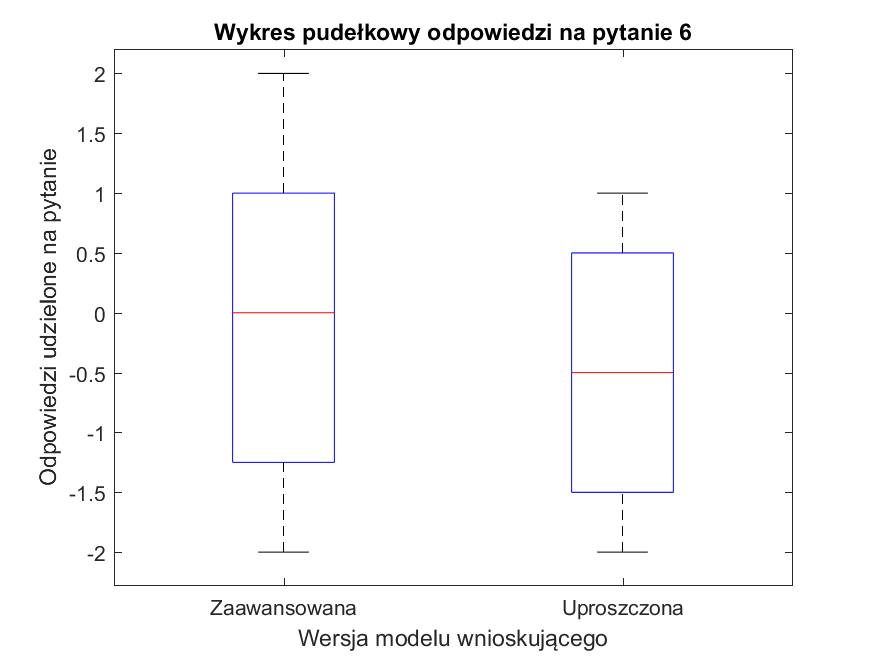
\includegraphics[scale=0.8]{rozdzial5/Ewaluacja6.png}
		\caption{Ewaluacja: pytanie 6 -- wykres pudełkowy.}
	\end{figure}
	
	\subsubsection{Obserwacje i wnioski:}
	
	Zarówno niniejsze pytanie, jak i to o nieodpowiednich momentach, wskazują, że system owszem był delikatnie uciążliwy, bo każde przerywanie i zadawanie pytań jest uciążliwe. Z drugiej jednak strony generalnie oceny użytkowników są raczej wysokie, więc plugin w wersji zaawansowanej został przygotowany jako przyjazny dla użytkowników. Należy też odnotować, że system okazał się bardziej uciążliwy dla użytkowników wersji prostej.
	
	
	
\subsection{Czy system NIE zabierał mi zbyt dużo czasu?}
	
	\subsubsection{Cel pytania:}
	
	Jednym z celów rozszerzenia \textit{HowAreYou} było zmniejszenie uciążliwości odpytywania użytkownika, między innymi przez stworzenie prostego, intuicyjnego i jak najbardziej nieinwazyjnego interfejsu. Pytanie weryfikuje tę funkcjonalność.
	
	W podobnych ankietach często ludzie pomijają słowo nie, dlatego zostało ono dodatkowo wyróżnione.
	
	\subsubsection{Uzyskane wyniki:}
	
	\begin{table}[!h]
		\caption{Ewaluacja: pytanie 7 -- uzyskane wyniki.}
		\centering
		\begin{tabular}{|c|c|c|c|c|c|c|c|c|c|c|c|c|c|}
			\hline
			Wersja &  \multicolumn{9}{c|}{Zaawansowana} & \multicolumn{4}{c|}{Uproszczona}\\ \hline
			Identyfikator użytkownika             & 1 & 2 & 3 & 4 & 5 & 6 & 7 & 8 & 9 
			& 10 & 11 & 12 & 13 \\ \hline
			Odpowiedzi poszczególnych uczestników & -2 & -1 & -1 & 0 & 1 & -1 & 1 & 0 & -1
			& -1 & 0 & 1 & -2     \\ \hline
		\end{tabular}
	\end{table}
	
	\begin{table}[!h]
		\caption{Ewaluacja: pytanie 7 -- prosta analiza statystyczna.}
		\centering
		\begin{tabular}{|c|c|c|}
			\hline
			Wersja          & Zaawansowana & Uproszczona \\ \hline
			Wartość średnia & -0.44        & -0.50       \\ \hline
			Wariancja       &  1.03        &  1.67       \\ \hline
			Mediana         & -1.00        & -0.50       \\ \hline
		\end{tabular}
	\end{table}
	
	\begin{figure}[H]
		\centering
		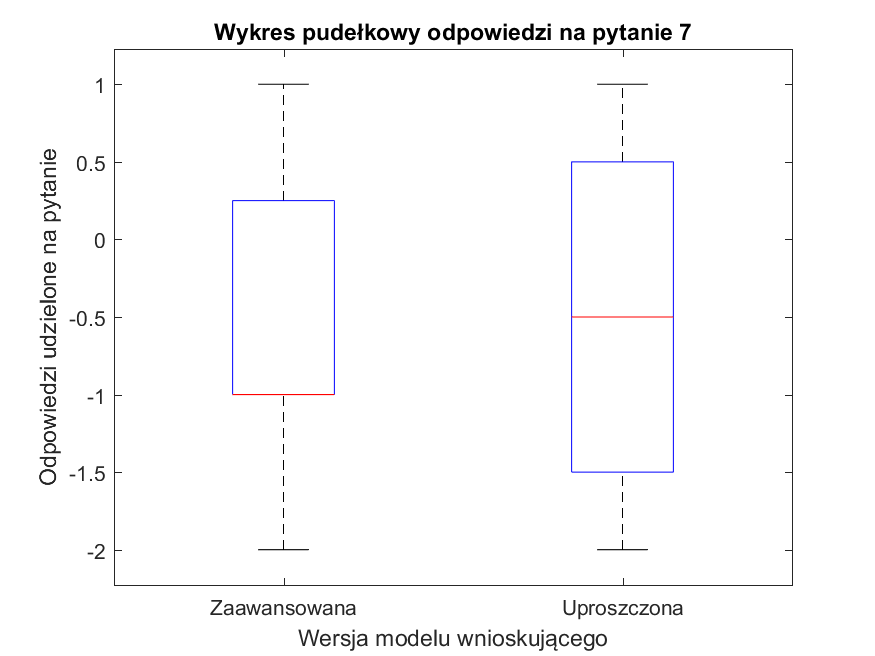
\includegraphics[scale=0.8]{rozdzial5/Ewaluacja7.png}
		\caption{Ewaluacja: pytanie 7 -- wykres pudełkowy.}
	\end{figure}
	
	\subsubsection{Obserwacje i wnioski:}
	
	Pomimo tego, że w jednym z poprzednich pytań spora część użytkowników wskazała, że była pytana w nieodpowiednich momentach, czy też że system przeszkadzał im w korzystaniu z telefonu, w tej kwestii użytkownicy byli raczej zgodni -- w większości określili system jako nieczasochłonny.
	
	
	
\subsection{Czy skanowanie nastroju z wykorzystaniem kamery telefonu było dla mnie zauważalne?}
	
	\subsubsection{Cel pytania:}
	
	Celem analizowania nastroju poprzez wykonywanie fotografii było ograniczenie uciążliwości działania systemu poprzez przeniesienie części odpowiedzialności z jawnego odpytywania na niejawne skanowanie. W teorii -- skanowanie nie powinno być zauważalne dla użytkownika. Pytanie dodano, aby tę hipotezę potwierdzić. Zadano je tylko tym uczestnikom badania, którzy wykorzystywali funkcjonalność kamery w wersji rozszerzonej.
	
	\subsubsection{Uzyskane wyniki:}
	
	\begin{table}[!h]
		\caption{Ewaluacja: pytanie 8 -- uzyskane wyniki.}
		\centering
		\begin{tabular}{|c|c|c|c|c|c|c|c|c|c|c|c|c|c|}
			\hline
			Wersja &  \multicolumn{9}{c|}{Zaawansowana} & \multicolumn{4}{c|}{Uproszczona}\\ \hline
			Identyfikator użytkownika             & 1 & 2 & 3 & 4 & 5 & 6 & 7 & 8 & 9 
			& 10 & 11 & 12 & 13 \\ \hline
			Odpowiedzi poszczególnych uczestników & -1 & -2 & 0 & 0 & -1 & -2 & -1 & 1 & -1
			& --  & -- & -- & -- \\ \hline
		\end{tabular}
	\end{table}
	
	\begin{table}[!h]
		\caption{Ewaluacja: pytanie 8 -- prosta analiza statystyczna.}
		\centering
		\begin{tabular}{|c|c|c|}
			\hline
			Wersja          & Zaawansowana & Uproszczona \\ \hline
			Wartość średnia & -0.78        & --          \\ \hline
			Wariancja       &  0.94        & --          \\ \hline
			Mediana         & -1.00        & --          \\ \hline
		\end{tabular}
	\end{table}
	\clearpage
	
	\begin{figure}[H]
		\centering
		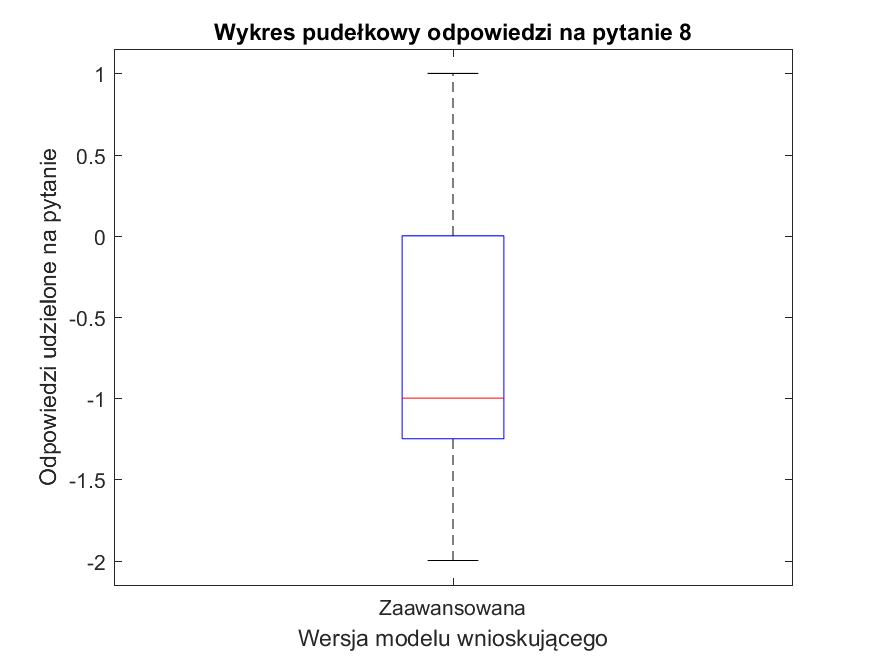
\includegraphics[scale=0.8]{rozdzial5/Ewaluacja8.png}
		\caption{Ewaluacja: pytanie 8 -- wykres pudełkowy.}
	\end{figure}
	
	\subsubsection{Uzyskane wyniki -- wersja uproszczona:}
	
	Nie dotyczy.
	
	\subsubsection{Obserwacje i wnioski:}
	
	Większość użytkowników wskazała, że podczas kilkudniowego badania wykorzystywanie kamery telefonu nie było dla nich zauważalne. 
	
	
	
\subsection{Czy skanowanie nastroju z wykorzystaniem kamery telefonu wpływało na moje codzienne zachowanie? Czy mogłoby być na dłuższą metę uciążliwe?}
	
	\subsubsection{Cel pytania:}
	
	Celem pytania było zbadanie, jak świadomość bycia fotografowanym wpływa na uczestnika badania. Chodziło także o zestawienie tego pytania z poprzednim -- o zauważalność skanowania.
	
	\subsubsection{Uzyskane wyniki:}
	
	\begin{table}[!h]
		\caption{Ewaluacja: pytanie 9 -- uzyskane wyniki.}
		\centering
		\begin{tabular}{|c|c|c|c|c|c|c|c|c|c|c|c|c|c|}
			\hline
			Wersja &  \multicolumn{9}{c|}{Zaawansowana} & \multicolumn{4}{c|}{Uproszczona}\\ \hline
			Identyfikator użytkownika             & 1 & 2 & 3 & 4 & 5 & 6 & 7 & 8 & 9 
			& 10 & 11 & 12 & 13 \\ \hline
			Odpowiedzi poszczególnych uczestników & 1 & 2 & 1 & 1 & 0 & 1 & -1 & -1 & 1
			& -- & -- & -- & --     \\ \hline
		\end{tabular}
	\end{table}
	
	\begin{table}[!h]
		\caption{Ewaluacja: pytanie 9 -- prosta analiza statystyczna.}
		\centering
		\begin{tabular}{|c|c|c|}
			\hline
			Wersja          & Zaawansowana & Uproszczona \\ \hline
			Wartość średnia & 0.56         & --          \\ \hline
			Wariancja       & 1.03         & --          \\ \hline
			Mediana         & 1.00         & --          \\ \hline
		\end{tabular}
	\end{table}
	
	\begin{figure}[H]
		\centering
		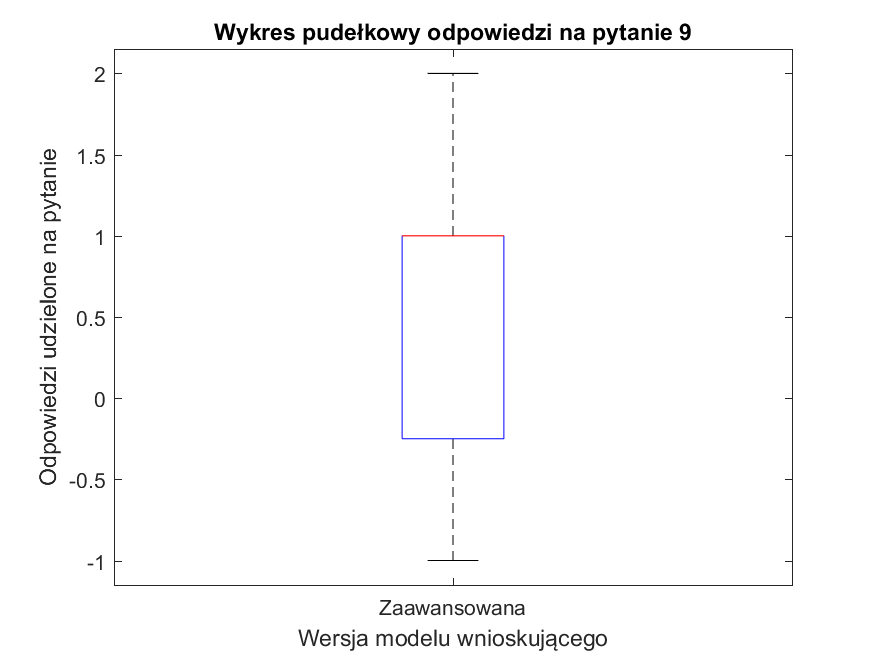
\includegraphics[scale=0.8]{rozdzial5/Ewaluacja9.png}
		\caption{Ewaluacja: pytanie 9 -- wykres pudełkowy.}
	\end{figure}
	
	\subsubsection{Obserwacje i wnioski:}
	
	Pomimo, że w poprzednim pytaniu większość uczestników wskazała, że przy kilkudniowym badaniu samo skanowanie nastroju nie było dla nich zauważalne, to jednak miało ono wpływ na ich codzienne zachowanie. To naturalne -- każdy człowiek chroni swoją prywatność. Taka świadomość bycia podglądanym wymusza na nas pewne zmiany.
	
	
\subsection{Czy system działał zgodnie z konfiguracją i z moimi oczekiwaniami?}
	
	\subsubsection{Cel pytania:}
	
	Celem pytania było sprawdzenie oceny działania systemu przez użytkowników, abstrahując od kwestii wygody czy uciążliwości. Chodziło o sprawdzenie niezawodności i ewentualnie możliwości konfiguracji systemu.
	
	\subsubsection{Uzyskane wyniki:}
	
	\begin{table}[!h]
		\caption{Ewaluacja: pytanie 10 -- uzyskane wyniki.}
		\centering
		\begin{tabular}{|c|c|c|c|c|c|c|c|c|c|c|c|c|c|}
			\hline
			Wersja &  \multicolumn{9}{c|}{Zaawansowana} & \multicolumn{4}{c|}{Uproszczona}\\ \hline
			Identyfikator użytkownika             & 1 & 2 & 3 & 4 & 5 & 6 & 7 & 8 & 9 
			& 10 & 11 & 12 & 13 \\ \hline
			Odpowiedzi poszczególnych uczestników & 1 & 2 & 1 & 0 & 1 & 2 & 1 & 1 & 2
			& -1 & 1 & 0 & 1    \\ \hline
		\end{tabular}
	\end{table}
	
	\begin{table}[!h]
		\caption{Ewaluacja: pytanie 10 -- prosta analiza statystyczna.}
		\centering
		\begin{tabular}{|c|c|c|}
			\hline
			Wersja          & Zaawansowana & 0.25        \\ \hline
			Wariancja       & 0.44         & 0.92        \\ \hline
			Mediana         & 1.00         & 0.50        \\ \hline
		\end{tabular}
	\end{table}
	
	\begin{figure}[H]
		\centering
		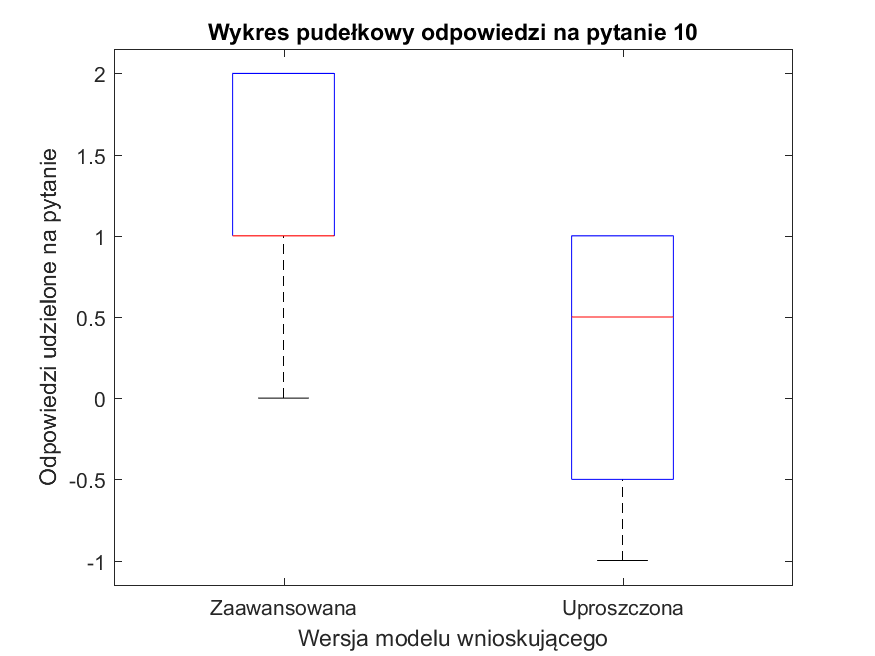
\includegraphics[scale=0.8]{rozdzial5/Ewaluacja10.png}
		\caption{Ewaluacja: pytanie 10 -- wykres pudełkowy.}
	\end{figure}
	
	\subsubsection{Obserwacje i wnioski:}
	
	Działanie pluginu \textit{HowAreYou} zostało przez użytkowników ocenione dobrze. System zebrał same oceny pozytywne i neuralne dla wersji rozszerzonej i tylko jedną negatywną dla prostego odpytywania z~wykorzystaniem widoku emotikon.
	
	